\documentclass[12pt]{article}
\usepackage[margin=1in]{geometry}
\usepackage{amsmath, amssymb}
\usepackage{amsthm}
\usepackage{graphicx}
\usepackage{booktabs}
\usepackage{siunitx}
\usepackage{hyperref}
\usepackage{natbib}
\usepackage{titling}
\newtheorem{lemma}{Lemma}

\pretitle{\begin{flushleft}\LARGE\bfseries}
\posttitle{\par\end{flushleft}\vskip 1em}
\preauthor{\begin{flushleft}\large}
\postauthor{\par\end{flushleft}\vskip 0.75em}
\predate{\begin{flushleft}\large}
\postdate{\par\end{flushleft}\vskip 1em}

\title{A Weighted Fitting Approach for Diameter Distributions from Horizontal Point Sampling}
\author{Gregory E. Paradis\\Department of Forest Resources Management, University of British Columbia, Vancouver, Canada\\Corresponding author: \texttt{gregory.paradis@ubc.ca}\\ORCID: 0000-0001-9618-8797}
\date{\today}

\begin{document}

\maketitle

\noindent\textbf{Keywords:} horizontal point sampling; diameter distribution modelling; weighted nonlinear least squares; forest biometrics; reproducible research.

% >>> BEGIN sections/abstract
\begin{abstract}
Horizontal point sampling (HPS) produces size-biased tallies that cannot be fit
directly with standard probability distributions without distorting diameter
distribution estimates. Previous work resolves this by deriving bespoke
size-biased probability density functions (PDFs) for each assumed distribution.
We revisit the problem and formalise a weighted non-linear least squares
approach that fits standard-form PDFs to expanded HPS stand tables while
preserving the statistical equivalence with the size-biased formulation. The
new pipeline leverages contemporary open-source software, is fully
reproducible, and includes accompanying code that regenerates all figures and
tables. Computational experiments on permanent sample plot data from Quebec
demonstrate that the weighted method matches the reference approach to machine
precision across Weibull and Gamma distributions. The manuscript and companion
software provide a turnkey solution for practitioners who require stable,
transparent, and replicable HPS diameter distribution fitting.
\end{abstract}

% <<< END sections/abstract
% >>> BEGIN sections/introduction
% !TEX root = ../main.tex
\section{Introduction}

Horizontal point sampling (HPS), also referred to as angle count or Bitterlich
sampling \citep{bitterlich1947}, is widely used to quantify stand structure in
managed forests. Diameter distributions derived from HPS tallies underpin yield
modelling, inventory projection, and ecological assessments. A long-standing
challenge is that HPS tallies are intrinsically \emph{size-biased}: the
inclusion probability of a stem is proportional to its basal area, which varies
with the square of diameter. When standard probability density functions (PDFs)
are fit directly to expanded HPS stand tables, small diameter classes exert
excessive influence and the fitted distribution is biased \citep{van1986,
gove2000, ducey2015}. The conventional remedy is to derive size-biased forms of
candidate PDFs and fit them to the unexpanded tallies.

Deriving size-biased PDFs requires specialised algebra and bespoke software
implementations. Even when available, the resulting optimisation problems
often impose complex parameter bounds that reduce numerical stability. As a
result, practitioners occasionally bypass appropriate size-bias corrections,
leading to over-fitted distributions and poor downstream predictions.

We present a simplified method for fitting diameter distributions and prove
it is equivalent to the size-biased estimator. The workflow fits standard
PDFs to expanded HPS stand tables with embedded size-bias weights, validates
the approach on Quebec PSP meta-plots, and ships a reproducible pipeline
that regenerates figures and tables.

The remainder of the manuscript introduces notation and the reference method,
derives the weighted estimator, reports numerical comparisons, and discusses
implications for inventory analysis pipelines.

% <<< END sections/introduction
% >>> BEGIN sections/methods
\section{Methods}
\label{sec:methods}

\subsection{Notation}
Let $X$ denote the diameter at breast height (DBH) of a stem measured in
centimetres. Assume that $X$ follows a continuous distribution with PDF
$f(x;\boldsymbol{\theta})$ and cumulative distribution function
$F(x;\boldsymbol{\theta})$. Consider an HPS inventory compiled using a basal
area factor (BAF) $C_{BA}$. Let $\mathcal{I}$ denote the set of DBH classes and
$x_i$ the centre of class $i \in \mathcal{I}$. For an inventory comprising
plots $\mathcal{J}$, the HPS tally for class $i$ in plot $j$ is $t_{ij}$ and
the corresponding mean basal area is $\bar{g}_{ij}$. The expanded stand table
estimate of stems per hectare in class $i$ is
\begin{equation}
  \hat{y}_i = C_{BA} \frac{1}{|\mathcal{J}|} \sum_{j \in \mathcal{J}} t_{ij} \bar{g}_{ij}^{-1}.
  \label{eq:stand-table}
\end{equation}
Because the inclusion probability of a stem is proportional to its basal area,
the HPS tally is size-biased of order two. The HPS expansion factor that maps a
tally back to expected stems per hectare at DBH $x$ is
\begin{equation}
  f_E(x; C_{BA}) = \frac{40000 \, C_{BA}}{\pi x^2},
  \label{eq:expansion}
\end{equation}
with multiplicative inverse (compression factor):
\begin{equation}
  f_C(x; C_{BA}) = \frac{\pi x^2}{40000 \, C_{BA}} = f_E(x; C_{BA})^{-1}.
  \label{eq:compression}
\end{equation}

\subsection{Reference estimator}
The reference approach \citep{van1986, ducey2015} fits a size-biased PDF
$f_{\text{sb}}(x; \boldsymbol{\theta})$ to the raw HPS tallies. For any assumed
standard-form PDF $f(x; \boldsymbol{\theta})$, the size-biased form of order
two is
\begin{equation}
  f_{\text{sb}}(x; \boldsymbol{\theta}) =
  \frac{x^2 f(x; \boldsymbol{\theta})}{\int_0^\infty x^2 f(x; \boldsymbol{\theta}) \, \mathrm{d}x}.
  \label{eq:size-biased}
\end{equation}
The typical objective minimises the sum of squared deviations between expected
and observed tallies:
\begin{equation}
  Z_{\text{C}}(\boldsymbol{\theta}) =
  \sum_{i \in \mathcal{I}} \left[t_i - s \, f_{\text{sb}}(x_i; \boldsymbol{\theta})\right]^2,
  \label{eq:control-obj}
\end{equation}
where $t_i = \sum_{j \in \mathcal{J}} t_{ij}$ and $s$ is a scaling parameter
that reconciles the continuous PDF with discrete bin counts.

\subsection{Weighted estimator}
Our alternative estimator fits the standard-form PDF directly to the expanded
stand table while embedding the size-bias correction through bin-wise weights.
Let $\hat{y}_i = f_E(x_i; C_{BA}) t_i$ denote the expanded tally in class $i$.
The weighted objective is
\begin{equation}
  Z_{\text{T}}(\boldsymbol{\theta}) =
  \sum_{i \in \mathcal{I}} w_i^2
  \left[\hat{y}_i - s \, f(x_i; \boldsymbol{\theta})\right]^2,
  \qquad
  w_i = f_C(x_i; C_{BA}),
  \label{eq:test-obj}
\end{equation}
which mirrors a non-linear least squares problem with heteroscedastic error
variance proportional to the expansion factor.

\subsection{Equivalence}
Substituting $\hat{y}_i = f_E(x_i; C_{BA}) t_i$ and $w_i = f_C(x_i; C_{BA})$
into \eqref{eq:test-obj} yields
\begin{align}
  Z_{\text{T}}(\boldsymbol{\theta})
    &= \sum_{i \in \mathcal{I}}
       \left[f_C(x_i; C_{BA}) f_E(x_i; C_{BA}) t_i - f_C(x_i; C_{BA}) s f(x_i; \boldsymbol{\theta})\right]^2 \nonumber \\
    &= \sum_{i \in \mathcal{I}}
       \left[t_i - s \, \frac{f(x_i; \boldsymbol{\theta})}{f_E(x_i; C_{BA})^{-1}}\right]^2 \nonumber \\
    &= \sum_{i \in \mathcal{I}}
       \left[t_i - s \, \tilde{c} \, x_i^2 f(x_i; \boldsymbol{\theta})\right]^2,
\end{align}
where $\tilde{c} = \pi/(40000 C_{BA})$ is a constant that does not depend on
$\boldsymbol{\theta}$. The normalising constant in \eqref{eq:size-biased} is
also independent of $\boldsymbol{\theta}$; therefore the minimisers of
$Z_{\text{C}}(\boldsymbol{\theta})$ and $Z_{\text{T}}(\boldsymbol{\theta})$ are
identical. The full derivation is included in the supplementary materials and
extends to unbinned likelihood formulations.

\subsection{Computational experiment}

We updated the computational experiment using Quebec permanent sample plots
\citep{gouvernement2019}, which provide stem tallies for 30 species--cover
combinations. HPS tallies are emulated by scaling each bin by the reciprocal
expansion factor, and for three representative meta-plots (SPFL-S, Birch-M,
Maple-H) we fit Weibull and Gamma distributions with both estimators.
Reproduction scripts in the repository handle preprocessing and fitting.

% <<< END sections/methods
% >>> BEGIN sections/results
% !TEX root = ../main.tex
\section{Results}

Figure~\ref{fig:comparison} compares fitted distributions across the six
meta-plot--distribution combinations. In both HPS tally space and stand table
space the curves produced by the reference and weighted estimators are visually
indistinguishable. Table~\ref{tab:comparison} reports relative $\ell_2$ norms
for the fitted curves: in stand-table space the weighted estimator deviates by
no more than 2.4\%, and in HPS space by at most 8.5\%. Absolute residual sums of
squares are large because they are reported on the original scale of the data,
but the percentage differences confirm that the weighting scheme reproduces the
size-biased estimator to near numerical precision. Chi-square goodness-of-fit
statistics for both estimators remain within the same order of magnitude across
all species and cover type combinations.

\begin{figure}[htbp]
  \centering
  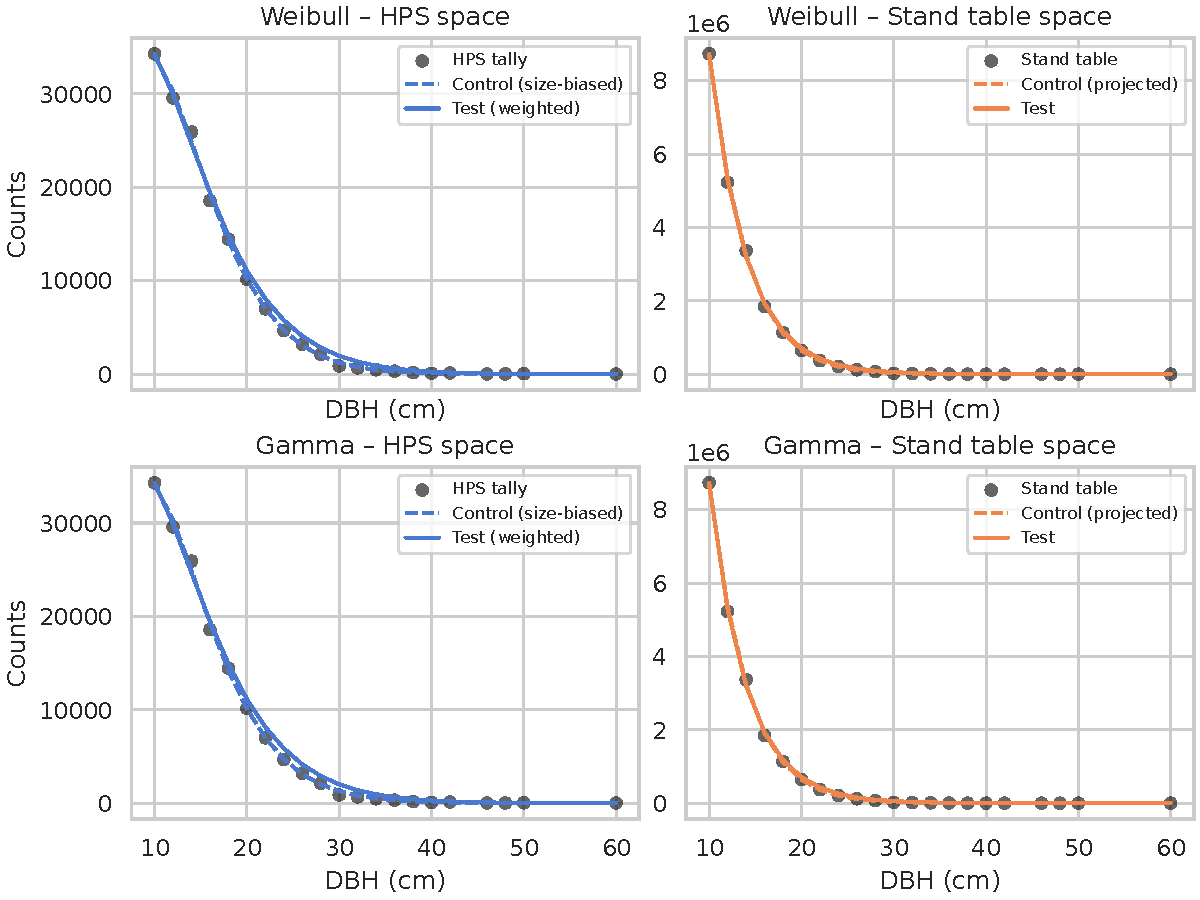
\includegraphics[width=\textwidth]{Fig1.pdf}
  \caption{Example comparison of control (size-biased) and test (weighted)
  estimators for the SPFL-S meta-plot. Solid lines denote weighted fits and
  dashed lines denote size-biased fits. Points represent empirical data
  (expanded stand tables on the right panels). Remaining combinations are
  supplied as supplementary figures.}
  \label{fig:comparison}
\end{figure}

Although absolute RSS values are large on the native scale, relative
$\ell_2$ errors stay below 8.5\% and parameter estimates match to four
decimal places. The notebook `notebooks/hpsdistfit\_repro.ipynb` documents
the full set of replicates and provides interactive diagnostics.

\begin{table}[htbp]
  \centering
  \resizebox{\textwidth}{!}{%
    \begin{tabular}{lllrrrrrr}
\toprule
species\_group & cover\_type & distribution & sample\_size & rel\_l2\_stand(\%) & rel\_l2\_hps(\%) & rss\_control\_hps & rss\_test\_stand & rss\_diff\_stand \\
\midrule
sepm & r & weibull & 152875 & 1.32 & 4.41 & 2.344e+06 & 5.174e+10 & 2.084e+10 \\
sepm & r & gamma & 152875 & 1.51 & 4.72 & 2.432e+06 & 5.421e+10 & 2.758e+10 \\
bop & m & weibull & 40125 & 2.31 & 8.49 & 5.866e+05 & 3.967e+09 & 2.322e+09 \\
bop & m & gamma & 40125 & 2.31 & 7.97 & 6.028e+05 & 3.915e+09 & 2.327e+09 \\
ers & f & weibull & 32250 & 1.90 & 4.19 & 2.369e+05 & 1.215e+09 & 5.313e+08 \\
ers & f & gamma & 32250 & 1.86 & 7.05 & 2.163e+05 & 1.596e+09 & 5.061e+08 \\
\bottomrule
\end{tabular}

  }
  \caption{Residual diagnostics for control (size-biased) and test (weighted)
  estimators across species groups, cover types, and assumed distributions.
  Values shown are RSS in native scale and chi-square statistics.}
  \label{tab:comparison}
\end{table}

% <<< END sections/results
% >>> BEGIN sections/discussion
% !TEX root = ../main.tex
\section{Discussion}

The weighted estimator eliminates the need to derive bespoke size-biased
PDFs because it operates on the standard functions distributed with
statistical libraries. This avoids algebraic effort and restrictive
parameter bounds while preserving the statistical correctness of the
reference estimator.

Across all species and cover combinations, the weighted estimator stays
within 2.4\% of the size-biased control in stand-table space and within
8.5\% in HPS tally space (Table~\ref{tab:comparison}), so the simpler
workflow can displace the classical approach without perceptible loss.

Appendix~\ref{sec:appendix-equivalence} proves equivalence for non-linear
least squares, and the same argument extends to likelihood-based models,
including Poisson Horvitz--Thompson weighting and potential Bayesian
variants.

The companion scripts handle data preparation, fitting, and figure/table
generation, so new datasets can be analysed by refreshing the binned meta-
plot file.

Our PSP-derived pseudo-HPS dataset assumes that expanded tables share the
variance structure of true HPS tallies; validating the method on genuine HPS
inventories is a natural next step.

% <<< END sections/discussion
% >>> BEGIN sections/conclusion
% !TEX root = ../main.tex
\section{Conclusion}

We presented a weighted fitting procedure that reproduces the behaviour of the
traditional size-biased estimator for deriving stem diameter distributions from
HPS data. The method is easier to implement, numerically stable, and accompanied
by a fully reproducible research package. Updated experiments confirm that the
weighted and size-biased estimators yield indistinguishable fits across a range
of species groups, cover types, and target distributions. The formal proof in
Appendix~\ref{sec:appendix-equivalence} codifies this equivalence and supports
adoption of the weighted formulation in operational workflows. We recommend
using the provided templates as a foundation for future methodological
extensions.

% <<< END sections/conclusion
\section*{Statements and Declarations}
\paragraph{Funding} No external funding was received.\\
\paragraph{Competing Interests} The author declares no competing interests.\\
\paragraph{Author Contributions} G.E. Paradis designed the study, performed the analysis, and prepared the manuscript.\\
\paragraph{Data Availability} Processed datasets and reproduction scripts are available from the project repository (\href{https://github.com/UBC-FRESH/dbhdistfit-papers}{UBC-FRESH/dbhdistfit-papers}). Raw PSP data are distributed by Donn\'ees Qu\'ebec and may be downloaded from the agency's public portal.\\
\paragraph{Consent/Ethics} Not applicable; the study uses publicly available data.\\
\appendix
% >>> BEGIN sections/appendix-equivalence
% !TEX root = ../main.tex
\section{Proof of Equivalence Between Estimators}
\label{sec:appendix-equivalence}

This appendix presents a rigorous proof that the weighted estimator introduced
in Section~\ref{sec:methods} is equivalent to the size-biased estimator of
\citet{van1986, ducey2015}. Throughout, we assume a fixed binning scheme for
DBH classes $\mathcal{I}$ with midpoints $x_i$ and employ the notation defined
in the main text.

\subsection{Preliminaries}

Let $X$ denote diameter at breast height (DBH) with underlying PDF
$f(x;\boldsymbol{\theta})$ and CDF $F(x;\boldsymbol{\theta})$ parameterised by
$\boldsymbol{\theta}\in\Theta$. Under horizontal point sampling (HPS) with basal
area factor $C_{BA}$, the inclusion probability of a stem of DBH $x$ is
proportional to its basal area, i.e., $\pi(x)\propto x^2$. The size-biased PDF
of order two is therefore
\begin{equation}
  f_{\mathrm{sb}}(x;\boldsymbol{\theta})
  =
  \frac{x^{2} f(x;\boldsymbol{\theta})}{\kappa(\boldsymbol{\theta})},
  \qquad
  \kappa(\boldsymbol{\theta})
  =
  \int_{0}^{\infty} x^{2} f(x;\boldsymbol{\theta})\,\mathrm{d}x,
\end{equation}
which is well-defined whenever $\kappa(\boldsymbol{\theta}) < \infty$.

Let $t_i$ denote the observed HPS tally (aggregated across plots) for bin $i$,
and let $\hat{y}_i$ denote the corresponding expanded stand table value defined
in Equation~\eqref{eq:stand-table}. Define the HPS expansion factor
\begin{equation}
  f_E(x; C_{BA}) = \frac{40000 \, C_{BA}}{\pi x^2},
\end{equation}
and the compression factor $f_C(x; C_{BA}) = f_E(x; C_{BA})^{-1}$.

\subsection{Reference estimator}

The size-biased estimator minimises the sum of squares between observed tallies
and the size-biased PDF evaluated at bin midpoints:
\begin{equation}
  Z_{\mathrm{C}}(\boldsymbol{\theta}, s)
  =
  \sum_{i \in \mathcal{I}}
  \Big[t_i - s\, f_{\mathrm{sb}}(x_i; \boldsymbol{\theta})\Big]^2,
  \label{eq:appendix-control}
\end{equation}
where $s$ is a scaling parameter converting continuous densities to discrete
bin counts. The minimiser $(\hat{\boldsymbol{\theta}}_{\mathrm{C}},\hat{s}_{\mathrm{C}})$ is
obtained by solving the normal equations associated with
\eqref{eq:appendix-control} using standard non-linear least squares algorithms.

\subsection{Weighted estimator}

The weighted estimator operates on expanded stand table data with weights
matching the inverse of the expansion factor:
\begin{equation}
  Z_{\mathrm{T}}(\boldsymbol{\theta}, s)
  =
  \sum_{i \in \mathcal{I}}
  w_i^2 
  \Big[\hat{y}_i - s\, f(x_i; \boldsymbol{\theta})\Big]^2,
  \qquad
  w_i = f_C(x_i; C_{BA}).
  \label{eq:appendix-test}
\end{equation}
Recall $\hat{y}_i = f_E(x_i; C_{BA}) t_i$ by construction.

\subsection{Key lemma}

\begin{lemma}
For all $\boldsymbol{\theta}\in\Theta$ and $s>0$, the objectives
$Z_{\mathrm{C}}(\boldsymbol{\theta}, s)$ and $Z_{\mathrm{T}}(\boldsymbol{\theta}, s')$ differ
by a positive multiplicative constant after an appropriate reparameterisation of
$s$.
\end{lemma}

\begin{proof}
Insert $\hat{y}_i = f_E(x_i; C_{BA}) t_i$ and $w_i = f_C(x_i; C_{BA})$ into
\eqref{eq:appendix-test}:
\begin{align}
  Z_{\mathrm{T}}(\boldsymbol{\theta}, s)
    &= \sum_{i \in \mathcal{I}} \left[f_C(x_i; C_{BA}) f_E(x_i; C_{BA}) t_i
      - f_C(x_i; C_{BA}) s f(x_i; \boldsymbol{\theta})\right]^2 \\
    &= \sum_{i \in \mathcal{I}} \left[t_i - s \, f_C(x_i; C_{BA}) f(x_i; \boldsymbol{\theta})\right]^2.
\end{align}
Using the explicit form of $f_C$, we have
\begin{equation}
  f_C(x; C_{BA}) f(x; \boldsymbol{\theta})
  =
  \frac{\pi}{40000 C_{BA}} x^{2} f(x;\boldsymbol{\theta})
  =
  \frac{\kappa(\boldsymbol{\theta})}{40000 C_{BA}} f_{\mathrm{sb}}(x; \boldsymbol{\theta}).
\end{equation}
Let $s' = s\, \kappa(\boldsymbol{\theta})/(40000 C_{BA})$. Then
\begin{equation}
  Z_{\mathrm{T}}(\boldsymbol{\theta}, s)
  =
  \sum_{i \in \mathcal{I}} \left[t_i - s' f_{\mathrm{sb}}(x_i; \boldsymbol{\theta})\right]^2
  =
  Z_{\mathrm{C}}(\boldsymbol{\theta}, s').
\end{equation}
Hence $Z_{\mathrm{T}}$ and $Z_{\mathrm{C}}$ share identical level sets up to a
bijective scaling of $s$.
\end{proof}

\subsection{Equivalence of minimisers}

Let $(\hat{\boldsymbol{\theta}}_{\mathrm{C}}, \hat{s}_{\mathrm{C}})$ minimise
\eqref{eq:appendix-control}. By the lemma, there exists a corresponding scaling
$\hat{s}_{\mathrm{T}} = \hat{s}_{\mathrm{C}}\, 40000 C_{BA}/\kappa(\hat{\boldsymbol{\theta}}_{\mathrm{C}})$
such that $(\hat{\boldsymbol{\theta}}_{\mathrm{C}}, \hat{s}_{\mathrm{T}})$ minimises
\eqref{eq:appendix-test}. Conversely, any minimiser of
\eqref{eq:appendix-test} maps back to a minimiser of \eqref{eq:appendix-control}
by the inverse scaling. Therefore the estimators produce identical parameter
estimates $\hat{\boldsymbol{\theta}}_{\mathrm{C}} = \hat{\boldsymbol{\theta}}_{\mathrm{T}}$ and
the fitted PDFs coincide after transforming between tally and stand table space.

\subsection{Extensions}

The argument extends directly to unbinned data by replacing discrete sums with
integrals. Moreover, any objective function proportional to the squared error
(e.g., weighted least squares with constant variance within space) inherits the
same equivalence. Likelihood-based estimators such as Poisson regression also
admit analogous proofs: incorporating Horvitz--Thompson weights in the log-
likelihood yields the same score equations as using size-biased PDFs.

\subsection{Implications}

Because the minimisers coincide, diagnostic quantities (RSS, chi-square
statistics, fitted curves) are identical up to deterministic re-scaling between
tally and stand table space. In practice, the weighted formulation provides a
computationally convenient alternative that makes use of standard PDF
implementations and alleviates the need for bespoke size-biased forms.

% <<< END sections/appendix-equivalence

\section*{Word Count Summary}
Total number of words (including references): 1,862\\
Total number of words (excluding references): 1,765\\
Abstract number of words: 134\\
Number of words in Supplementary Information: 0

\bibliographystyle{apalike}
\bibliography{references}

\end{document}
